\title{Android -- Eine Einführung}
\subtitle{Einstellungen, SQLite, Dateisystem \& ContentProvider}
\author[A. Wilhelm]{Andreas Wilhelm}
\institute[www.avedo.net]{}
\titlegraphic{}
%\date{\today}
\date{CSC Computer-Schulung \& Consulting GmbH}

\begin{frame}[plain]
  \titlepage
\end{frame}

\section[Contents]{}
\begin{frame}
	\frametitle{Contents}
	\tableofcontents[onlyparts]
\end{frame}

\part{Einstellungen}
\frame{\partpage}
\begin{frame}
	\frametitle{Contents}
	\tableofcontents[]
\end{frame}

\section{Überblick}
\begin{frame}
   \frametitle{Überblick}
   \begin{itemize}
      \item Anpassung von Verhalten und Aussehen der Applikation durch den 
         Anwender
      \item Erstellung von Oberflächen mit Android \emph{Preference}-API 
      \item Deklaration von Einstellungen mit XML
      \item Zugriff auf Einstellungen mit \emph{SharedPreferences}
      \item Darstellung mit PreferenceActivity bzw. -Fragment
      \item Ableiten eigener Einstellungen
   \end{itemize}

   \begin{alertblock}{PreferenceActivity}
      Bis Android 3.0 wurden Einstellungen über eine von \emph{PreferenceActivity} 
      abgeleitete Aktivität angezeigt. Seit Android 3.0 verwendet man 
      vorzugsweise \emph{PreferenceFragments}.
   \end{alertblock}

   \begin{table}[t]
      \begin{center}
         \begin{tabular}{c|c|c}
            Boolean & Float & Int\\
            \hline
            Long & String & String Set\\
         \end{tabular}
         \label{tab:preference_types}
         \caption{Typen von Einstellungen}
      \end{center}
   \end{table}
\end{frame}

\section{Deklaration in XML}
\begin{frame}
   \frametitle{Überblick}
   \begin{itemize}
      \item Deklaration in XML-Datei (\emph{res/xml/})
      \item Alternativ können Einstellungen auch zur Laufzeit hinzugefügt werden
      \item Wurzelknoten muss ein \emph{PreferenceScreen} sein
      \item Unterhalb des Wurzelnkotens Verschachtelung von \emph{Preference} Objekten
   \end{itemize}

   \begin{attrDesc}{+p{4cm}|^p{6cm}}
      Klasse & Beschreibung\\
      \hline
      \emph{CheckBoxPreference} & Checkbox-Eintrag - Einstellungen mit boolschem Wert\\
      \emph{EditTextPreference} & Einstellungen als Text\\
      \emph{ListPreference} & Auswahlliste mit nur einer wählbaren Option\\
      \emph{MultiSelectListPreference} & Auswahlliste mit mehreren wählbaren Optionen\\
      \emph{SwitchPreference} & Speichern eines boolschen Werts\\
      \emph{RingtonePreference} & Auswahl eines der auf dem Gerät verfügbaren Klingeltöne\\
      \emph{DialogPreference} & Dialog über den Einstellungen vorgenommen werden können\\
      \emph{PreferenceCategory} & Gruppiert Einstellungen unter gemeinsamen Abschnitt\\
      \emph{PreferenceScreen} & Gruppiert Einstellungen unter gemeinsamen Menüpunkt\\
   \end{attrDesc}
\end{frame}

\begin{frame}
   \frametitle{Attribute}
   \begin{attrDesc}{+p{4cm}|^p{6cm}}
      Attribut & Beschreibung\\
      \hline
      \emph{android:key} & Schlüssel über den Einstellung erreicht werden kann. 
         Anders als sonst üblich wird hier keine Android-ID sondern eine Zeichenkette verwendet. 
      	Elemente, die nicht vom Typ \emph{PreferenceCategory} der \emph{PreferenceScreen} 
      	sind oder ein Intent oder ein Fragment starten, müssen diesen Wert setzen.\\
      \emph{android:title} & Der Titel der Einstellung\\
      \emph{android:summary} & Ein kurzer Text mit Zusatzinformationen\\
      \emph{android:defaultValue} & Der voreingestellte Standard-Wert dieser Einstellung\\
      \emph{android:fragment} & Deklariert ein anzuzeigendes Fragment\\
   \end{attrDesc}
\end{frame}

\begin{frame}
   \frametitle{Beispiel}
   \lstinputlisting[
      language=xml,caption=Deklaration der Einstellungen,
      label={lst:preferences.xml}]{src/xml/preferences.xml}
\end{frame}

\begin{frame}
   \frametitle{Screenshots}
   \begin{figure}[h!]
     \centering
     \subfigure[Startansicht der Einstellungen]{
        \includegraphics[width=0.47\textwidth]{pictures/preferences.ps}
        \label{fig:preferencestart}
     }\hfill
     \subfigure[Der Datetime PreferenceScreen]{
        \includegraphics[width=0.47\textwidth]{pictures/preference_list.ps}
        \label{fig:preferencescreen}
     }
     \caption{
        Die Einstellungen
     }
     \label{fig:preferences}
   \end{figure}
\end{frame}

\section{Verwenden von Intents}
\begin{frame}
   \frametitle{Überblick}
   \begin{itemize}
      \item Direkte Verwendung von \emph{Preference}
      \item Deklaration eines impliziten Intents
   \end{itemize}

   \begin{attrDesc}{+p{4cm}|^p{6cm}}
      Attribut & Beschreibung\\
      \hline
      \emph{android:action} & Die Aktion, die das Intent auslösen soll\\
      \emph{android:data} & Daten, die über das Intent weitergegeben werden sollen\\
      \emph{android:mimeType} & Der zu verwendende MIME Typ\\
      \emph{android:targetClass} & Der Name der Zielklasse (der Aktivität)\\
      \emph{android:targetPackage} & Der Paket der Zielklasse (der Aktivität)\\
   \end{attrDesc}
\end{frame}

\begin{frame}
   \frametitle{Implementierung}
   \lstinputlisting[
      language=xml,caption=Einstellungen und Intents,
      label={lst:preference_intent.xml}]{src/xml/preference_intent.xml}
\end{frame}

\begin{frame}
   \frametitle{Screenshots}
   \begin{figure}[h!]
     \centering
     \subfigure[Der Intent-Eintrag in den Einstellungen]{
        \includegraphics[width=0.47\textwidth]{pictures/preference_intent.ps}
        \label{fig:preference_intent_item}
     }\hfill
     \subfigure[Die Seite im Browser]{
        \includegraphics[width=0.47\textwidth]{pictures/preference_intent_clicked.ps}
        \label{fig:preference_intent_clicked}
     }
     \caption{
        Einstellungen und Intents
     }
     \label{fig:preference_intent}
   \end{figure}
\end{frame}


\section{Preference Aktivitäten \& Fragmente}
\begin{frame}
   \frametitle{PreferenceActivity}
   \begin{itemize}
      \item Bis Android 3.0 Einsatz von \emph{PreferenceActivity}
      \item Laden der Einstellungen in \emph{onCreate()}
      \item Zuweisen eines Layouts nicht nötig
      \item Einstellungen werden automatisch gespeichert
      \item Dynamisches Laden mit \emph{findPreference()}
   \end{itemize}

   \lstinputlisting[
      caption=Implementierung einer PreferenceActivity,
      label={lst:SettingsActivity.java}]{src/java/SettingsActivity.java}
\end{frame}

\begin{frame}
   \frametitle{PreferenceFragment}
   \begin{itemize}
      \item Seit Android 3.0 Einsatz von \emph{PreferenceFragments}
      \item Implementierung wie bei \emph{PreferenceActivity}
   \end{itemize}

   \lstinputlisting[
      caption=Implementierung eines PreferenceFragments,
      label={lst:SettingsFragment.java}]{src/java/SettingsFragment.java}
\end{frame}

\begin{frame}
   \frametitle{Laden der Fragments}
   \lstinputlisting[
      caption=Einbinden des PreferenceFragments,
      label={lst:SettingsActivity2.java}]{src/java/SettingsActivity2.java}
\end{frame}

\section{Standard-Einstellungen setzen}
\begin{frame}
   \frametitle{Überblick}
   \begin{itemize}
      \item Setzen von Standard-Werten für \emph{SharedPreferences}
      \item Zuweisung über Attribut \emph{android:defaultValue}
      \item Initialisierung mit \emph{setDefaultValues()} in allen \emph{onCreate()} 
      	Methoden von Aktivitäten, die als Einstiegspunkte dienen
   \end{itemize}

   \lstinputlisting[
      caption=Initialisierung der SharedPreferences,
      label={lst:setDefaultValues.java}]{src/java/setDefaultValues.java}

   \begin{alertblock}{Die Methode setDefaultValues()}
      Die Methode \emph{setDefaultValues()} nimmt drei Argumente entgegen. 
      Die ersten beiden sind der Kontext und die Deklaration 
      der Einstellungen, die in den SharedPreferences initialisiert werden sollen. 
      Der dritte Wert legt allerdings fest, ob die bisherigen Benutzereinstellungen 
      überschrieben werden sollen oder nicht. Steht dieser Wert auf \emph{true} 
      werden alle bisherigen Einstellungen des Benutzers gelöscht und mit den 
      Standard-Einstellungen überschrieben.
   \end{alertblock}
\end{frame}

\section{Einstellungen Kategorisieren}
\begin{frame}
   \frametitle{Überblick}
   \begin{itemize}
      \item Umfangreiche Einstellungen recht unübersichtlich
      \item Bisher Lösung durch verschachtelte \emph{PreferenceScreens}
      \item Seit Android 3.0 Lösung über \emph{Header}
      \item Vorteil: Header erzeugen auf größeren Bildschirmen ein Zwei-Spalten-Layout
   \end{itemize}

   \lstinputlisting[
      language=xml,caption=Einstellungen kategorisieren,
      label={lst:preference_headers.xml}]{src/xml/preference_headers.xml}
\end{frame}

\begin{frame}
   \frametitle{Laden der Header}
   \lstinputlisting[
      caption=Initialisierung der SharedPreferences,
      label={lst:SettingsHeaders.java}]{src/java/SettingsHeaders.java}
\end{frame}

\begin{frame}
   \frametitle{Hinweis}
   \begin{alertblock}{Kompatibilität}
		Da Header erst in Android 3.0 eingeführt wurden, muss man eine gesonderte Behandlung 
		für ältere Geräte einfügen. Anhand der Version können unterschiedliche Deklarationen 
		der Einstellungen geladen werden (siehe Listing~\ref{lst:SettingsHeaders.java}). 
		Die Methode \emph{onBuildHeaders()} wird dann in älteren Versionen einfach ignoriert.
   \end{alertblock}
\end{frame}

\begin{frame}
   \frametitle{Generische Fragments}
   \begin{itemize}
      \item Bisher Deklaration einzelner Fragments
      \item Implementierung eines generischen Fragments
      \item Übergabe von Inhalten mit \emph{\textless{}extras\textgreater}-Element
   \end{itemize}

   \lstinputlisting[
      language=xml,caption=Einstellungen kategorisieren,
      label={lst:preference_header_extras.xml}]{src/xml/preference_header_extras.xml}
\end{frame}

\begin{frame}
   \frametitle{Behandlung von generischen Fragments}
   \lstinputlisting[
      caption=Laden der Preferences,
      label={lst:SettingsFragment2.java}]{src/java/SettingsFragment2.java}
\end{frame}

\section{Einstellungen lesen}
\begin{frame}
   \frametitle{Überblick}
   \begin{itemize}
      \item Einstellungen einer Applikation werden in einer Datei gespeichert
      \item Zugriff über Klasse \emph{SharedPreferences} 
      \item Verwaltung durch \emph{PreferenceManager}
      \item Laden mit Methode \emph{getDefaultSharedPreferences()} 
   \end{itemize}

   \lstinputlisting[
      caption=Laden der Einstellungen,
      label={lst:SharedPreferences.java}]{src/java/SharedPreferences.java}
\end{frame}

\begin{frame}
   \frametitle{Aktualisierungen}
   \begin{itemize}
      \item Änderungen in Einstellungen nicht sofort berücksichtigt
      \item Implementierung eines Listeners
   \end{itemize}

   \lstinputlisting[
      caption=Reagieren auf Änderungen an den Einstellungen,
      label={lst:OnSharedPreferenceChangeListener.java}]{src/java/OnSharedPreferenceChangeListener.java}
\end{frame}
   
\section{Eigene Einstellungen implementieren}
\begin{frame}
   \frametitle{Überblick}
   \begin{itemize}
      \item Grundlegende Einstellungswidgets in Android enthalten
      \item Weitere Widgets können selbst implementiert werden
      \item Beispiel: NumberPicker
      \item Typischerweise Ableitung von \emph{DialogPreference}
      \item Bei Ableitung von \emph{Preference} Implementierung von \emph{onClick()} 
      	Methode
   \end{itemize}
\end{frame}

\begin{frame}
   \frametitle{NumberPickerPreference}
   \lstinputlisting[
      caption=Konstruktor des Einstellungselements,
      label={lst:DialogPreference.java}]{src/java/DialogPreference.java}
\end{frame}

\begin{frame}
   \frametitle{Speichern der Einstellung}
   \begin{itemize}
      \item Speichern der Einstellungen mit \emph{persist*()} Methoden  
      \item Automatisches Übertragen in \emph{SharedPreferences}
   \end{itemize}

   \lstinputlisting[
      caption=Speichern der Einstellungen,
      label={lst:onDialogClosed.java}]{src/java/onDialogClosed.java}
\end{frame}

\begin{frame}
   \frametitle{Laden der Einstellung}
   \begin{itemize}
      \item Initialisierung mit Methode \emph{onSetInitialValue()}
      \item Laden von Einstellung mit Methode \emph{getPersisted*()} 
   \end{itemize}

   \lstinputlisting[
      caption=Laden der Einstellungen,
      label={lst:onSetInitialValue.java}]{src/java/onSetInitialValue.java}

   \begin{alertblock}{Standard-Wert}
      Man kann den an die Methode \emph{onSetInitialValue()} übergebenen Standard-Wert 
      nicht verwenden, denn falls das Flag \emph{restorePersistedValue} gesetzt wurde, 
      ist dieser Wert automatisch \emph{null}.
   \end{alertblock}
\end{frame}

\begin{frame}
   \frametitle{Setzen des Standard-Werts}
   \begin{itemize}
      \item Implementierung des Setzens mit \emph{android:defaultValue} 
         über Methode \emph{onGetDefaultValue()}
      \item Auch wenn Methode Standard-Wert übergeben bekommt muss 
         eigener Wert bereitgestellt werden
   \end{itemize}

   \lstinputlisting[
      caption=Laden der Standard-Einstellungen,
      label={lst:onGetDefaultValue.java}]{src/java/onGetDefaultValue.java}
\end{frame}

\begin{frame}
   \frametitle{Speichern des aktuellen Status}
   \begin{itemize}
      \item Einstellungen gehen beim Neustart (Rotation des Geräts) 
         verloren
      \item Methode \emph{onSaveInstanceState()} speichert aktuellen 
         Status
      \item Methode \emph{onRestoreInstanceState()} lädt aktuellen 
         Status
   \end{itemize}

   \lstinputlisting[
      caption=Speichern und Laden des aktuellen Status,
      label={lst:preferenceInstanceState.java}]{src/java/preferenceInstanceState.java}
\end{frame}

\begin{frame}
   \frametitle{Den Status verwalten}
   \begin{itemize}
      \item Implementierung durch Ableitung von \emph{Preference.BaseSavedState}
      \item Überschreiben einiger Methoden
      \item Implementierung eines Creators
   \end{itemize}

   \begin{alertblock}{Standard-Wert}
      Ein Creator ist eine Klasse, die das \emph{Creator} Interface implementiert. 
      Sie müssen in einer Klasse, die das Parcelable Interface implementiert, als 
      öffentlich zugreifbares Feld \emph{CREATOR} hinterlegt werden, dass dazu verwendet wird 
      Instanzen dieser Klasse von einem \emph{Parcel} zu erzeugen.
   \end{alertblock}
\end{frame}

\begin{frame}
   \frametitle{Eine eigene Status Klasse}
   \lstinputlisting[
      caption={Das NumberPicker Status-Objekt}]{src/java/NumberPickerState.java}
\end{frame}

\part{Interner Speicher}
\frame{\partpage}
\begin{frame}
	\frametitle{Contents}
	\tableofcontents[]
\end{frame}

\section{Überblick}
\begin{frame}
   \frametitle{Allgemeines}
   \begin{itemize}
      \item Dateien im internen Speicher meistens nur von erstellenden Applikation 
      	nutzbar
      \item Dateien werden beim Deinstallieren der Applikation gelöscht
      \item Schreiben und Lesen von Dateien über Java-Streams
      \item Öffnen der Streams über Kontext der Applikation (\emph{openFileOutput()} und 
			\emph{openFileInput()})
   \end{itemize}
\end{frame}

\section{Datei-Operationen}
\begin{frame}
   \frametitle{Datei schreiben}
   Beim Öffnen des Ausgabe-Streams mit \emph{openFileOutput()} 
   muss ein Datei-Modus angegeben werden:
   
   \begin{attrDesc}{+p{4cm}|^p{6cm}}
      Attribut & Beschreibung\\
      \hline
      \emph{MODE\_PRIVATE} & Erstellt Datei oder ersetzt existierende Datei, 
      	die nur für Applikation zugreifbar ist\\
      \emph{MODE\_APPEND} & Fügt Text am Ende einer existierenden Datei ein\\
      \emph{MODE\_WORLD\_READABLE} & Erlaubt allen Applikationen das Lesen der Datei\\
      \emph{MODE\_WORLD\_WRITEABLE} & Erlaubt allen Applikationen das Schreiben der Datei\\
   \end{attrDesc}

	\lstinputlisting[
		caption=Eine interne Datei beschreiben,
		label={lst:writeInternalFile.java}]{src/java/writeInternalFile.java}
\end{frame}

\begin{frame}
   \frametitle{Datei lesen}
   \begin{itemize}
      \item Dateien werden mit \emph{FileInputStreams} gelesen
      \item Einziger Parameter Name der Datei
      \item Blockweise Verarbeitung
   \end{itemize}

	\lstinputlisting[
		caption=Eine interne Datei lesen,
		label={lst:readInternalStorage.java}]{src/java/readInternalStorage.java}

	\begin{alertblock}{Statische Text-Resourcen}
		Größere Texte, wie eine Dokumentation oder Hilfe, können 
		als Resourcen hinterlegt werden. Dazu können beliebige Dateien im Ordner 
		\emph{res/raw/} gespeichert und mit \emph{Ressources.openRawResource()}, 
		unter Angabe der ID \emph{R.raw.\textless{}filename\textgreater}, geladen werden.
	\end{alertblock}
\end{frame}

\section{Erweiterungen}
\begin{frame}
   \frametitle{Cache-Dateien}
   \begin{itemize}
      \item Normaler Datei-Zugriff
      \item Methode \emph{getCacheDir()} liefert Zielordner von Cache-Dateien 
      \item System kann Cache-Dateien jeder Zeit löschen
      \item Cache-Dateien werden bei Deinstallation der Applikation gelöscht
   \end{itemize}
\end{frame}

\begin{frame}
   \frametitle{Erweiterte Datei-Zugriffe}
	\begin{attrDesc}{+p{4cm}|^p{6cm}}
		Methode & Beschreibung\\
		\hline
		\emph{getFilesDir()} & Liefert absoluten Pfad zum internen Dateisystem\\
		\emph{getDir()} & Öffnet oder erstellt ein Verzeichnis im internen 
			Speicherbereich\\
		\emph{deleteFile()} & Löscht eine Datei aus dem internen Speicher\\
		\emph{fileList()} & Gibt \emph{File}-Array der aktuell durch die Applikation 
			im internen Speicher abgelegten Dateien zurück
	\end{attrDesc}

	\begin{alertblock}{File-Methoden}
		Zudem stehen natürlich die Methoden der \emph{File}-Klasse, 
		wie \emph{isDirectory()} und \emph{canRead()} zur Verfügung.
	\end{alertblock}
\end{frame}

\part{Externer Speicher}
\frame{\partpage}
\begin{frame}
	\frametitle{Contents}
	\tableofcontents[]
\end{frame}

\section{Überblick}
\begin{frame}
   \frametitle{Allgemeines}
   \begin{itemize}
      \item Externer Speicher vom Gerät abhängig
      \item Kann als interner und SD-Speicher vorliegen
      \item Bei SD-Speicher muss unbedingt Verfügbarkeit geprüft werden
      \item Verwaltet privaten und öffentlichen Speicher
      \item Zugriff über \emph{getExternalFilesDir()} oder \emph{getExternalStoragePublicDirectory()}
      \item Zugriff über selbst erzeugten Input- und OutputStream
   \end{itemize}
   
	\lstinputlisting[
		caption=Externen Speicher überprüfen,
		label={lst:checkExternalState.java}]{src/java/checkExternalState.java}
\end{frame}

\begin{frame}
   \frametitle{Privater Speicher}
   \begin{itemize}
   	\item Enthält nur Dateien der Applikation
   	\item Wird beim Deinstallieren gelöscht
      \item \emph{getExternalFilesDir()} erwartet Typ des zu öffnenden Verzeichnisses
      \item Typ ist Datei abhängig, Beispiel \emph{Context.DIRECTORY\_MUSIC}
      \item Dateien können so von Android-Media-Scanner gefunden werden
      \item Android-Media-Scanner stellt Dateien anderen Applikationen zur Verfügung
      \item Datei \emph{.nomedia} im Wurzelverzeichnis verhindert Durchsuchen 
      	durch Android-Media-Scanner
      \item \emph{getExternalFilesDir()} mit Parameter \emph{null} liefert 
      	Wurzelverzeichnis
   \end{itemize}
\end{frame}

\begin{frame}
   \frametitle{Öffentlicher Speicher}
   \begin{itemize}
   	\item Enthält öffentliche Dateien der Applikation
      \item Dateien sind für alle Applikationen les- und schreibbar
      \item Dateien bleiben auch nach Deinstallation gespeichert
      \item \emph{getExternalStoragePublicDirectory()} erwartet Typ des zu öffneden Verzeichnisses
      \item Typ ist Datei abhängig, Beispiel \emph{Context.DIRECTORY\_MUSIC}
   \end{itemize}

   \begin{attrDesc}{+p{4cm}|^p{6cm}}
		Ordner & Dateitypen\\
		\hline
		\emph{Music/} & Verschiedene Musik-Dateien.\\
		\emph{Podcasts/} & Podcasts.\\
		\emph{Ringtones/} & Musik und Sound-Dateien, die als Klingeltöne verwendet werden.\\
		\emph{Alarms/} & Signaltöne, die für Alarme verwendet werden.\\
		\emph{Notifications/} & Signaltöne, die für Notifikationen verwendet werden.\\
		\emph{Pictures/} & Alle Bilder, die nicht mit der Kamera aufgezeichnet wurden.\\
		\emph{Movies/} & Alle Videos, die nicht mit der Kamera aufgezeichnet wurden.\\
		\emph{Download/} & Dateien beliebigen Typs, die heruntergeladen wurden.\\
	\end{attrDesc}
\end{frame}

\section{Erweiterungen}
\begin{frame}
   \frametitle{Cache-Speicher}
   \begin{itemize}
   	\item Zugriff mit \emph{getExternalCacheDir()} 
   	\item Kann vom System jeder Zeit gelöscht werden
   	\item Wird bei Deinstallation gelöscht
   \end{itemize}

	\begin{alertblock}{Cache verwalten}
		Im Regelfall ist der externe Cache dem internen vorzuziehen, da einige 
		Endgeräte, wie beispielsweise das \emph{HTC Desire} nur einen sehr kleinen 
		internen Speicher mitbringen. Speichermangel, der zum Löschen der Applikation 
		durch den Benutzer führen könnte, wird so vermieden.
	\end{alertblock}
\end{frame}

\part{SQLite}
\frame{\partpage}
\begin{frame}
	\frametitle{Contents}
	\tableofcontents[]
\end{frame}

\section{Überblick}
\begin{frame}
   \frametitle{Allgemeines}
   \begin{itemize}
   	\item Standard Datenbank-System unter Android
   	\item Unterstützt alle gängigen Features von relationalen Datenbanken
   	\item \emph{SQL}-Syntax, \emph{Prepared Statement} und \emph{Transactions}
   	\item Infos unter \href{www.sqlite.org}{www.sqlite.org}
   	\item Zugriff unter Android nur durch erstellende Applikation
   	\item Erstellen einer Datenbank optimaler Weise mit \emph{SQLiteOpenHelper}
   	\item Methode \emph{onCreate()} erstellt Datenbank
   	\item Methode \emph{onUpgrade()} verwaltet Änderungen an Datenbank-Struktur
   \end{itemize}
\end{frame}

\begin{frame}
   \frametitle{Implementierung}
	\lstinputlisting[
		caption=Den SQLiteOpenHelper nutzen,
		label={lst:SQLiteOpenHelper.java}]{src/java/SQLiteOpenHelper.java}
\end{frame}

\section{SQLite-Abfragen}
\begin{frame}
   \frametitle{Datenbank-Zugriff}
   \begin{itemize}
   	\item Zugriff mit \emph{SQLiteDatabase}-Objekt 
   	\item Lesender Zugriff mit \emph{getReadableDatabase()} anfordern
   	\item Schreibender Zugriff mit \emph{getWriteableDatabase()} anfordern
   \end{itemize}

	\begin{alertblock}{SQLite-Tabellen}
		Android stellt keine Anforderungen an eine SQLite-Tabelle, 
		es empfiehlt sich jedoch in jeder Tabelle eine ID zu hinterlegen. 
		\emph{ContentProvider}, die auch anderen Programmen den Zugriff auf die in 
		dieser Datenbank hinterlegten Daten ermöglichen, fordern beispielsweise 
		einen solchen Schlüssel mit dem Namen \emph{\_ID}.
	\end{alertblock}
	
	\begin{alertblock}{Asynchroner Zugriff}
		Datenbank-Anfragen sind sehr langsam, da ein Zugriff auf das Dateisystem 
		nötig ist. Es empfiehlt sich seine Anfragen asynchron zur Applikation, 
		also in einem \emph{Thread} oder \emph{AsyncTask} auszuführen.
	\end{alertblock}  
\end{frame}

\begin{frame}
   \frametitle{Anfragen absetzen}
   \begin{itemize}
   	\item Direktes Ausführen einer Anfrage mit \emph{execSQL()}
   	\item Methoden \emph{insert()}, \emph{update()} und \emph{delete()} 
   		zum Einfügen, Ändern und Löschen von Datensätzen
   	\item \emph{query()} und \emph{rawQuery()} um Abfragen zu senden
   	\item Ergebnisse von Anfragen werden als \emph{Cursor}-Objekte zurückgeliefert
   \end{itemize}
\end{frame}

\section{Ergebnisse verarbeiten}
\begin{frame}
   \frametitle{Cursor}
   \begin{itemize}
   	\item \emph{Cursor} zeigt auf eine Zeile des Ergebnisses (nicht alle 
   		Zeilen werden in Speicher geladen)
   	\item \emph{moveToFirst()} schiebt Cursor an erste Position
   	\item \emph{moveToNext()} ermöglicht durchlaufen des Ergebnisses
   	\item Auf Ende mit Rückgabewert von \emph{moveToNext()} oder 
			direkt mit \emph{isAfterLast()} prüfen
   	\item Cursor stellt typenbasierte \emph{get*()} Methoden zur Verfügung
   	\item Beispiel: \emph{getString(columnIndex)}
   	\item Spalten-Index kann mit \emph{getColumnIndexOrThrow()} 
   		erfragt werden
   	\item Cursor immer mit \emph{close()} schließen
   \end{itemize}
\end{frame}

\begin{frame}
   \frametitle{Implementierung}
	\lstinputlisting[
		caption=SQLiteDatabase nutzen,
		label={lst:SQLiteDatabase.java}]{src/java/SQLiteDatabase.java}
\end{frame}

\begin{frame}
   \frametitle{Anmerkung}
   \begin{alertblock}{\emph{sqlite3} Werkzeug}
		Das Android SDK stellt das Werkzeug \emph{sqlite3} zur Verfügung, dass dazu verwendet 
		werden kann die Datenbanken direkt zu verwalten, wodurch Datenbank-Zugriffe 
		besser analysiert und Probleme schneller gefunden werden können.
	\end{alertblock}
\end{frame}

\part{ContentProvider}
\frame{\partpage}
\begin{frame}
	\frametitle{Contents}
	\tableofcontents[]
\end{frame}

\section{Überblick}
\begin{frame}
   \frametitle{Allgemeines}
   \begin{itemize}
   	\item Verwaltet den Zugriff auf zentral verfügbare Daten
   	\item Meistens Teil einer Applikation die selbst Zugriff auf diese Daten ermöglicht
   	\item Stellt anderen Applikationen einen oder mehrere Datenstämme (Tabellen)
   		zur Verfügung
   	\item Kontrolliert den Zugriff
   	\item Beispiel: \emph{Dictionary Provider} \& \emph{Contact Provider}
   	\item Zugriff über \emph{ContentResolver}-Objekt
   	\item Daten werden über \emph{URI} identifiziert
   	\item \emph{URI} setzt sich aus symbolischen Namen des Providers und einer 
			Tabelle zusammen
   \end{itemize}
\end{frame}

\section{Lesender Zugriff}
\begin{frame}
   \frametitle{ContentResolver}
   \begin{itemize}
   	\item Zugriffsmethoden (\emph{CRUD}-Methoden) zum Erstellen, Lesen, Ändern 
   		und Löschen der Daten
   	\item Anfrage über \emph{query()} Methode
   	\item Starke Ähnlichkeit zur SQL-Syntax
   	\item Liefert wie \emph{SQLite}-Bibliothek einen Cursor
   \end{itemize}
   
   \begin{attrDesc}{+p{4cm}|^p{6cm}}
		Parameter & Dateitypen\\
		\hline
		\emph{URI} & Identifiziert den ContentProvider und die durch ihn verwaltete Tabelle\\
		\emph{Spalten} & Enthält angeforderte Spaltennamen\\
		\emph{Auswahl Statement} & Deklariert einen SQL-\emph{WHERE} ähnliches Statement\\
		\emph{Auswahl Argumente} & Liefert die zur Auswahl benötigten Argumente\\
		\emph{Sortierung} & Legt eine Sortierung des Ergebnisses fest\\
	\end{attrDesc}
\end{frame}

\begin{frame}
   \frametitle{Beispiel}
	\lstinputlisting[
		caption=Einen ContentResolver nutzen,
		label={lst:dictionaryResolver.java}]{src/java/dictionaryResolver.java}
\end{frame}

\begin{frame}
   \frametitle{Implementierung}
   \begin{itemize}
   	\item Rechte werden im Android-Manifest gesetzt
   	\item Beispiel: \emph{android.permission.READ\_USER\_DICTIONARY}
   	\item Einbinden mit \emph{\textless{}uses-permission\textgreater}-Element
   \end{itemize}

	\lstinputlisting[
		language=sql,caption=Die SQL-Abfrage,
		label={lst:dictionarySql.sql}]{src/sql/dictionarySql.sql}
\end{frame}

\begin{frame}
   \frametitle{Implementierung II}

	\lstinputlisting[
		caption=Anfrage an einen ContentProvider,
		label={lst:dictionaryQuery.java}]{src/java/dictionaryQuery.java}
\end{frame}

\section{Datenverarbeitung}
\begin{frame}
   \frametitle{Ergebnisse Durchlaufen}
	\lstinputlisting[
		caption=Manuelles Durchlaufen des Cursors,
		label={lst:dictionaryCursor.java}]{src/java/dictionaryCursor.java}
\end{frame}

\begin{frame}
   \frametitle{Anzeigen von Ergebnissen}
	\lstinputlisting[
		caption=Verwendung des SimpleCursorAdapters,
		label={lst:dictionaryAdapter.java}]{src/java/dictionaryAdapter.java}
\end{frame}

\section{Verwaltung der Daten}
\begin{frame}
   \frametitle{Daten einfügen}
	\lstinputlisting[
		caption=Einfügen eines neuen Datensatzes,
		label={lst:dictionaryInsert.java}]{src/java/dictionaryInsert.java}
		
	\begin{alertblock}{Ergebnis-ID}
		Möchte man diese ID aus der URI extrahieren, so kann man dazu 
		\emph{ContentUris.parseId()} unter Angabe der URI aufrufen.
	\end{alertblock}
\end{frame}

\begin{frame}
   \frametitle{Daten ändern}
	\lstinputlisting[
		caption=Ändern von Datensätzen,
		label={lst:dictionaryUpdate.java}]{src/java/dictionaryUpdate.java}
\end{frame}

\begin{frame}
   \frametitle{Daten löschen}
	\lstinputlisting[
		caption=Löschen von Datensätzen,
		label={lst:dictionaryDelete.java}]{src/java/dictionaryDelete.java}
\end{frame}

\begin{frame}
   \frametitle{Zugriff über ID}
	\lstinputlisting[
		caption=Datensatz über URI ansprechen,
		label={lst:dictionaryDeleteById.java}]{src/java/dictionaryDeleteById.java}
   
   \begin{alertblock}{Asynchrone Anfragen}
	Alle Beispiele führen die Anfragen im Main-Thread aus. Da der Zugriff 
	über einen ContentResolver sehr langsam ist, ist es empfehlenswert 
	Anfragen asynchron, also in einem \emph{Thread} oder \emph{AsyncTask}, auszuführen.
	\end{alertblock}
\end{frame}

\section{Eigene ContentProvider}
\begin{frame}
   \frametitle{Allgemeines}
   \begin{itemize}
   	\item Ableiten einer Klasse von abstrakter Klasse \emph{ContentProvider}
   	\item Registrierung des ContentProviders im Manifest
   	\item Festlegen eines symbolischen Provider-Namens
   	\item Hinterlegen der Spaltennamen
   	\item Deklaration der Möglichen URIs
   	\item Alternativ können Konstanten auch in einer Contracts-Klasse 
   		implementiert werden
   	\item Hinterlegen der benötigten Zugriffsrechte
   \end{itemize}
\end{frame}

\begin{frame}
   \frametitle{Beispiel}
   
   Möglicher Provider-Name:\\
   \emph{net.avedo.ubuntu.releases.\textless{}provider\textgreater}\\
   
   Sich daraus ergebene URIs:
   \begin{itemize}
		\item content://net.avedo.ubuntu.releases.\textless{}provider\textgreater/\textless{}file\textgreater
		\item content://net.avedo.ubuntu.releases.\textless{}provider\textgreater/\textless{}table\textgreater
		\item content://net.avedo.ubuntu.releases.\textless{}provider\textgreater/\textless{}table\textgreater/\textless{}id\textgreater
	\end{itemize}
\end{frame}

\begin{frame}
   \frametitle{Basis-Methoden}
   \begin{itemize}
   	\item Erwartete Funktionen \emph{onCreate()}, \emph{insert()}, \emph{update()}, 
   		\emph{delete()}, \emph{query()} und \emph{getType()}
   	\item \emph{UnsupportedOperationException} sollte beispielsweise
   		schreibender Zugriff unterbunden werden
   	\item Alle Methoden außer \emph{onCreate()} können aus verschiedenen Threads 
   		aufgerufen werden\\
   		$\rightarrow$ Implementierung Thread-Safe
   	\item Keine längeren Operationen in \emph{onCreate()}
   	\item Nur bekannte Exceptions, wie \emph{UnsupportedOperationException}, 
   	\emph{NullPointerException} oder \emph{IllegalArgumentException} verwenden
   	\item \emph{getType()} liefert MIME Typ (\emph{text/html} oder \emph{image/jpeg})
   	\item Alternative: ''Entwickler-deklarierter'' (vendor-specific) MIME-Typ
	\end{itemize}
	
	Entwickler-deklarierte Typen haben die Formen:
	
   \begin{enumerate}
   	\item vnd.android.cursor.item/vnd.\textless{}provider\textgreater/\textless{}table\textgreater
   	\item vnd.android.cursor.dir/vnd.\textless{}provider\textgreater/\textless{}table\textgreater
   \end{enumerate}
\end{frame}

\begin{frame}
   \frametitle{Verarbeitung der URIs}
   \begin{itemize}
   	\item Verwendung von \emph{UriMatcher} zur Wildcard-Analyse
			\begin{description}
				\item[*] Sucht einen String aus beliebigen Zeichen und beliebiger Länge. 
				\item[\#] Sucht einen numerischen Wert beliebiger Länge. 
			\end{description}
   	\item Hinzufügen einer URI mit \emph{UriMatcher.match(uri)}
   	\item Beispiel: Unterscheidung zwischen Tabellen- und Datensatz-URI
   \end{itemize}
\end{frame}

\begin{frame}
   \frametitle{Android-Manifest}
   \begin{itemize}
   	\item Eintrag mit \emph{\textless{}provider\textgreater}-Element
   	\item Deklaration der Zugriffsrechte mit \emph{\textless{}permission\textgreater}-Elemente
   	\item Erlauben eines temporären Zugriffs mit \emph{android:grantUriPermssions} \emph{true}
   	\item Alternative: Gesteuerte Vergabe von temporärem Zugriff über 
   		\emph{\textless{}grant-uri-permission\textgreater}
   \end{itemize}
   
   \begin{attrDesc}{+p{4cm}|^p{6cm}}
		Attribut & Beschreibung\\
		\hline
		\emph{android:authorities} & Symbolischer Name des Providers, der diesen 
			innerhalb des Systems eindeutig identifiziert\\
		\emph{android:name} & Name der ContentProvider Klasse\\
		\emph{android:icon} & Icon für den Provider\\
		\emph{android:label} & Kurze Beschreibung des Providers\\
	\end{attrDesc}
\end{frame}

\begin{frame}
   \frametitle{Beispiel}
	\lstinputlisting[
		language=xml,caption=Provider und das Manifest,
		label={lst:provider_manifest.xml}]{src/xml/provider_manifest.xml}
\end{frame}
